\documentclass[10pt]{datasheet}

% Input encoding and typographical rules for English language
\usepackage{iftex}
\ifPDFTeX
    \usepackage[utf8]{inputenc}
\else
    \ifXeTeX
        \usepackage{fontspec}
    \fi
\fi

\usepackage[english]{babel}
\usepackage[iso,english]{isodate}
\usepackage{siunitx}

\usepackage{graphicx}
\usepackage{qrcode}

% These define global texts that are used in headers and titles.
\title{APQ Eurocard backplane}
\author{Patrick Baus, APQ}
\date{\today}
\newcommand{\versionNumber}{1.0.0}
\revision{Revision \versionNumber}
\companylogo{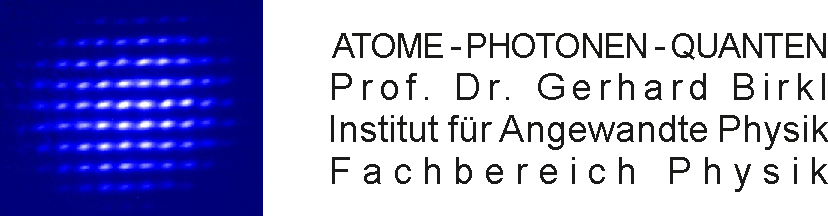
\includegraphics[width=55mm]{images/titel_apq-logo_cropped.pdf}}

\begin{document}
\maketitle

\section{Features}

\begin{itemize}
\item{Supports up to 6 eurocards with DIN 41612 type C connectors}
\item{Supports both open-frame and Fischer HB ME cases}
\item{Overvoltage and undervoltage protection}
\item{Reverse polarity protection up to \qty{\pm 48}{\V}}
\item{Soft-start and current limit with foldback}
\item{Transient voltage protection}
\item{\qtyrange{9}{24}{\V} @ \qty{12}{\A}}
\item{\qtyrange{-10}{-24}{\V} @ \qty{-12}{\A}}
\item Fully open-source design
\end{itemize}

\section{Applications}

\begin{itemize}
\item{Laser current drivers}
\item{Red Pitaya lockboxes}
\item{Laser temperature controllers}
\end{itemize}

\section{General Description}
The Eurocard backplane is compatible to several \qty{14}{HP} and \qty{28}{HP} rack mounted devices in the APQ device range. It is mounted in the rear of a \qty{3}{U} \qty{19}{''} subrack and supplies up to \num{6} devices with a bipolar \qty{\pm 15}{\V} (typical) voltage. The backplane can be used with most commercially available subrack chassis like the \href{https://www.fischerelektronik.de/web_fischer/en_GB/cases/N05.1/19%22%20subracks/$catalogue/fischerData/PR/BGT384_180/search.xhtml}{Fischer Elektronik BGT 384}.
Each slot can be configured to either hold devices enclosed in \href{https://www.fischerelektronik.com/web_fischer/en_GB/cases/N06.011/19%22%20insert%20modules/$catalogue/fischerData/PR/HBME14_/index.xhtml}{Fischer Elektronik HB ME 14}
modules or open-frame modules designed around the \href{https://www.fischerelektronik.com/web_fischer/en_GB/cases/N06.05/Part%20front%20panels/$catalogue/fischerData/PR/TFP14/index.xhtml}{Fischer Elektronik TFP 3 14}
front panels.
Six such modules with a width of \qty{14}{HP}, or up to 3 larger modules with width of \qty{28}{HP} can be installed. A mix of these is also possible as the backplane is configurable..

\begin{figure}[ht]
    \centering
    \includegraphics[width=7cm]{example-image}
\end{figure}

The backplane enables higher operating currents and better EMC protection when compared to air wired solutions and using \qty{2}{\milli\farad} of distributed capacitance allows to meet the increased performance requirements to ensure stable operation during most hot swapping events.

Additionally, the backplane features advanced input protection circuitry to safeguard against a variety of adverse conditions like overvoltage, undervoltage and short circuit events. It is designed to protect against hot-short situations where either rail is shorted to ground during operation.

The protection circuitry will shut down and restart the modules in an error event without exceeding the power limits or damage thresholds of either the power supply or the backplane.

The backplane is powered by a commercially available bench power supply to meet custom power limits and give a high degree of flexibility.

% Switch to next column
\vfill\break

% For wide tables, a single column layout is better. It can be switched
% page-by-page.
\onecolumn

\section{Revision History}
\begin{table}[h]
    \centering
    \begin{tabularx}{\textwidth}{l| l | >{\raggedright\arraybackslash}X}
        \thickhline
        Version& Date& Comment\\
        \hline
        1.0.0 &2023-10-19 & Initial release.\\
        \thickhline
    \end{tabularx}
\end{table}

The latest release of this document can be found at \url{https://github.com/TU-Darmstadt-APQ/DIN_41612_Backplane}.

\begin{center}
    \qrcode[nolinks]{https://github.com/TU-Darmstadt-APQ/DIN_41612_Backplane}
\end{center}

\clearpage
\section{Mechanical Specifications}
\begin{table}[h]
    \caption{}
    \begin{tabularx}{\textwidth}{l | c | X | c c c | c}
        \thickhline
        \textbf{Parameter} & \textbf{Symbol} & \textbf{Conditions} & \textbf{Min.} & \textbf{Typ.} & \textbf{Max.} &
        \textbf{Unit} \\
        \hline
        Board length  & $l_\text{h}$ & & 427.06 & 427.26 & 427.46 & \unit{\mm} \\
        Board width  & $l_\text{v}$ & & 128.35 & 128.55 & 128.75 & \unit{\mm} \\
        Board thickness  & $d$ & & 1.44 & 1.6 & 1.76 & \unit{\mm} \\
        \hline
        Copper thickness & $d_\text{Cu}$ & Copper is plated to \qty{2}{oz} on outer layer & & 70 & & \unit{\um} \\
        \hline
        Mating cycles & & Eurocard slot & 400 & & & \\
        \thickhline
    \end{tabularx}
\end{table}

\section{Electrical Specifications}
All specifications are for $\qty{-20}{\celsius} \leq T_A \leq \qty{60}{\celsius}$, unless otherwise noted.
\begin{table}[h!]
    \caption{}
    \begin{threeparttable}
        \begin{tabularx}{\textwidth}{l | c | X | c c c | c}
            \thickhline
            \textbf{Parameter} & \textbf{Symbol} & \textbf{Conditions} & \textbf{Min.} & \textbf{Typ.} & \textbf{Max.} &
            \textbf{Unit} \\
            \hline
            \multirow{3}{*}{Operating conditions}  & $V_\text{cc}$ &  & \num{8} & & \num{24} & \unit{\V} \\
            & $V_\text{ee}$ & (Note 1) & \num{-11} & & \num{-24} & \unit{V} \\
            & $I$ & (Note 1) & & & \num{\pm 12} & \unit{\A} \\
            \hline
            \multirow{2}{*}{Undervoltage threshold} & & (Note 2), $V_\text{cc} > V_\text{th}$, falling & \num{6.3} & \num{6.5} & \num{6.7} & \unit{\V} \\
             & & (Note 1, 2) & \num{-9.4} & \num{-10} & \num{-10.6} & \unit{\V} \\
            \multirow{2}{*}{Undervoltage hysteresis} & &(Note 2), $V_\text{cc} < V_\text{th}$, rising & \num{6.7} & \num{6.9} & \num{7.1} & \unit{\V} \\
             & & (Note 1, 2)  & \num{-8.8} & \num{-9.0} & \num{-9.3} & \unit{\V} \\
            \multirow{2}{*}{Overvoltage threshold} & & (Note 2), $V_\text{cc} < V_\text{th}$, rising & \num{25.6} & \num{26.1}& \num{26.7} & \unit{\V} \\
             & & (Note 1, 2) & \num{-25.9} & \num{-26.6}& \num{-27.3} & \unit{\V} \\
            \multirow{2}{*}{Overvoltage hysteresis} & & (Note 2), $V_\text{cc} > V_\text{th}$, falling & \num{24.7} & \num{25.3}& \num{25.9} & \unit{\V} \\
             & & (Note 1, 2) & \num{-24.7} & \num{-25.6}& \num{-26.5} & \unit{\V} \\
            \multirow{2}{*}{Overcurrent threshold} & & (Note 2) & \num{15} & \num{16.7} & \num{18} & \unit{\A} \\
             & & (Note 1, 2) & \num{-14.6} & \num{-16.7} & \num{-18.7} & \unit{\A} \\
            \hline
            \multirow{2}{*}{Current per pin} & & $T_\text{A} = \qty{20}{\celsius}$ & & & 1.5 & \unit{\A}\\
            & & $T_\text{A} = \qty{60}{\celsius}$ & & & 1.1 & \unit{\A}\\
            \multirow{2}{*}{Current per slot} & & $T_\text{A} = \qty{20}{\celsius}$ & & & 6 & \unit{\A}\\
            & & $T_\text{A} = \qty{60}{\celsius}$ & & & 4.4 & \unit{\A}\\
            \thickhline
        \end{tabularx}
        \begin{tablenotes}
            \item{\textbf{Note 1}: Value is treated as absolute value for the classification of min/max.}
            \item{\textbf{Note 2}: Specification is guaranteed by design and not \qty{100}{\percent} tested in production.}
        \end{tablenotes}
    \end{threeparttable}
\end{table}

\section{Absolute Maximum Ratings}

\begin{table}[h]
    \caption{}
    \begin{tabularx}{\textwidth}{l | X}
        \thickhline
        \textbf{Parameter} & \textbf{Rating} \hspace{5cm} \\
        \hline
        $V_\text{cc}$ & \qty{\pm 60}{\V} \\
        $V_\text{ee}$ & \qty{\pm 60}{\V} \\
        $I$ & \qty{\pm 20}{\A} \\
        Storage Temperature Range & \qtyrange{-20}{70}{\celsius}\\
        Operating Temperature Range & \qtyrange{-20}{60}{\celsius}\\
        \thickhline
    \end{tabularx}
\end{table}

\textbf{Note:} Stresses beyond those listed under \textit{Absolute Maximum Ratings} may cause permanent damage to the device. These are stress ratings only, which do not imply functional operation of the device at these or any other conditions beyond those indicated under \textit{Operating conditions}. Exposure to absolute-maximum-rated conditions for extended periods may affect device reliability.

\end{document}
